\subsection{Translational Controller}
The translational controllers follow a cascade structure, where the velocity is the inner loop and the position is the outer loop. The relation between the controllers is presented in \autoref{fig:cascade}.
%
\begin{figure}[H]
\centering
	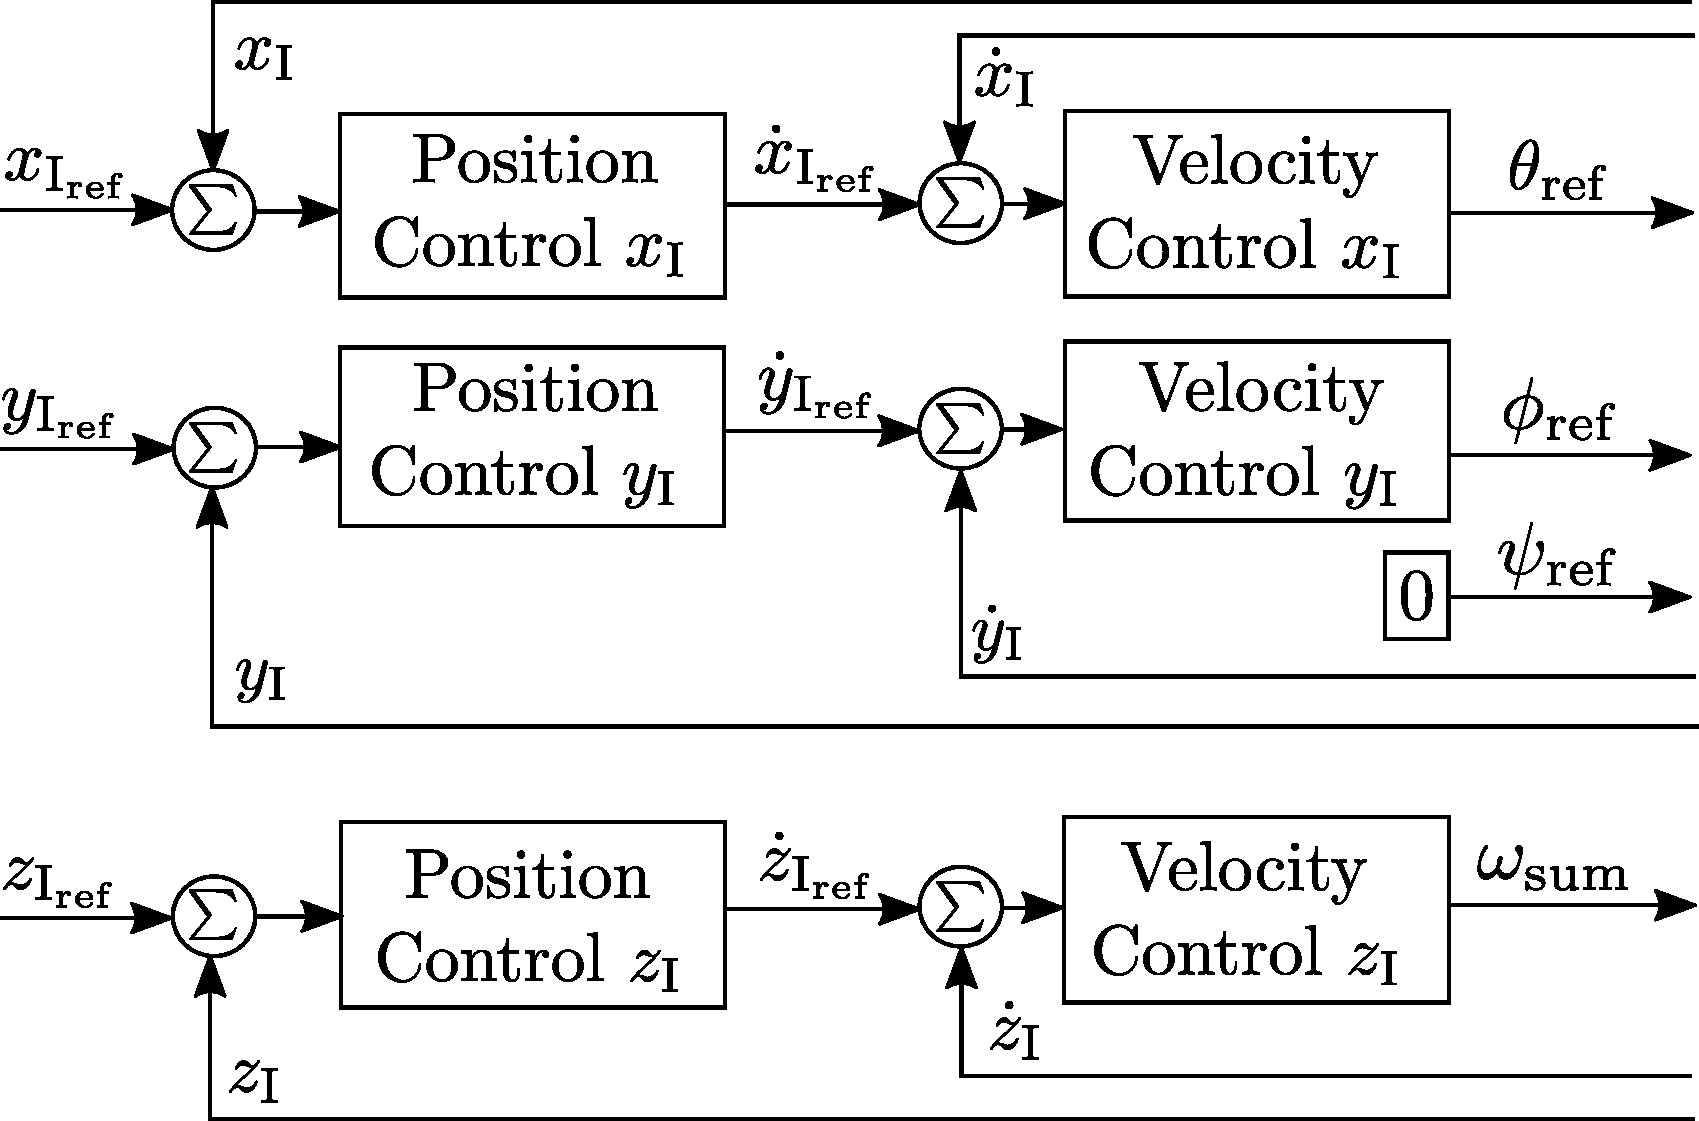
\includegraphics[width=.42\textwidth]{figures/TranslationalControlDiagramSmall.pdf}
	\caption{Overview of the translational controllers structure. $\overline{\omega}_{\mathrm{sum}}$ is the sum of rotational speeds requested by the $z_{\mathrm{I}}$ controller.}
	\label{fig:cascade}
\end{figure}
The $x_{\mathrm{I}}$ and $y_{\mathrm{I}}$ controllers share similar properties as both their outputs are angle references, $\theta_{\mathrm{ref}}$ and $\phi_{\mathrm{ref}}$. As the translational movement in $x_{\mathrm{I}}$ and $y_{\mathrm{I}}$ can be obtained by only changing these angles as long as $\psi$ is zero. For this reason, $\psi_{\mathrm{ref}}$ is set to zero all the time. The output of the $z_{\mathrm{I}}$ controller is the required sum of the motor rotational speeds.\\

In order to design the inner controllers for the velocities $\dot{x}_{\mathrm{I}}$, $\dot{y}_{\mathrm{I}}$ and $\dot{z}_{\mathrm{I}}$, the linear equations derived previously, see \autoref{eq:TransLinearEquations1}, \ref{eq:TransLinearEquations2} and \ref{eq:TransLinearEquations3}, are Laplace transformed. These are used to create the transfer functions, yielding
\begin{flalign}
    G_{\dot{x}}&=\frac{\dot{x}_{\mathrm{I}}}{\theta}=\frac{-k_{\mathrm{th}} (\overline{\omega}_1 ^2 + \overline{\omega}_2 ^2 + \overline{\omega}_3 ^2 + \overline{\omega}_4 ^2)}{m s} , \label{transferfunctionxdot} \\
    G_{\dot{y}}&=\frac{\dot{y}_{\mathrm{I}} }{\phi }=\frac{k_{\mathrm{th}}(\overline{\omega}_1 ^2 + \overline{\omega}_2 ^2 + \overline{\omega}_3 ^2 + \overline{\omega}_4 ^2)}{m s} , \label{transferfunctionydot} \\
    G_{\dot{z}}&=\frac{\dot{z}_{\mathrm{I}}}{\omega_{\mathrm{sum}}} = \frac{ -2 k_{\mathrm{th}}\overline{\omega}_{\mathrm{sum}} }{ 4m s } , \label{eq:linearTransferFunctionZ}
\end{flalign}

%\noindent where $G_{\dot{x}}$, $G_{\dot{y}}$ and $G_{\dot{z}}$  are the plants used to design the velocity controllers in $x_{\mathrm{I}}$, $y_{\mathrm{I}}$ and $z_{\mathrm{I}}$ directions respectively, $\omega_{\mathrm{sum}}$ is the sum of the rotational speeds of the motors and $\overline{\omega}_{\mathrm{sum}}$ is the sum of the rotational speeds in equilibrium.

The three plants contain an integrator that can handle steady state errors and output disturbances. However, if there are input disturbances, such as different motor characteristics or external causes like wind, an integrator term in the controller is needed. Then, a zero is added to remove the marginal stability due to the presence of only two integrators in the system. Finally, the gain is adjusted to reduce the oscillations. It is worth mentioning that, since the plants for the $x_{\mathrm{I}}$ and $z_{\mathrm{I}}$ velocities have a negative gain, the controller needs to compensate for it with a negative gain.

The bandwidth of the $\dot{x}_{\mathrm{I}}$, $\dot{y}_{\mathrm{I}}$ controllers is designed to be three times lower than that of the inner attitude controller. This reduces the influence of the attitude behavior on the outer velocity controller. The attitude controller has a bandwidth of 2 [\si{rad s^{-1}}], yielding a bandwidth of 0.7 [\si{rad s^{-1}}] for these two velocity controllers.

%Since the controllers for $\dot{x}_{\mathrm{I}}$, $\dot{y}_{\mathrm{I}}$ use the attitude controller as an inner loop to obtained the required angles, the bandwidth of the velocity controllers should therefore be considered. The gain is designed such that the system has a bandwidth that is three times lower than the attitude control loop. The attitude has a bandwidth of 2 rad s$^{-1}$, to reduce the effect of its dynamic in the velocity controllers. This yields a bandwidth of around 0.7 rad s$^{-1}$ for the velocity controllers in $x_{\mathrm{I}}$ and $y_{\mathrm{I}}$ directions.

 %\cite{bandwidthReference}.

The plants of the position control loops contain only an integrator, which transforms velocity to position. Since the disturbances are handled by the inner velocity controller, a proportional controller is used. In this case, there exists an inner loop in the three axes, so the consideration of the bandwidth has to be taken into count in all of them, making each bandwidth three times lower than that of the respective inner loop. Resulting in a bandwidth of 0.23 [\si{rad s^{-1}}] for the $x_{\mathrm{I}}$ and $y_{\mathrm{I}}$ controllers and 1 [\si{rad s^{-1}}] for the $z_{\mathrm{I}}$ controller.

%To be able to design the velocity loop for the z translational controller, the model equation derived previously, see \eqref{eq:TransLinearEquations3}, is Laplace transformed and written on the form of a transfer function, as
%%
%\vspace{-.1cm}
%%\begin{align}
%%G_{\dot{z}}=\frac{\dot{z}_{\mathrm{I}}}{\omega_{\mathrm{sum}}} &= \frac{ \frac{1}{4}(-2 k_{\mathrm{th}})\overline{\omega}_{\mathrm{sum}} }{ m s }\label{eq:linearTransferFunctionZ}
%%\end{align}
%
%%\noindent where $\dot{z}_\mathrm{I}$ is the velocity in the $z_{\mathrm{I}}$ direction, $\omega_{\mathrm{sum}}$ is the sum of the rotational speeds of the motors and $\overline{\omega}_{\mathrm{sum}}$ is the sum of the rotational speeds in equilibrium.
%
%Due to an integrator and a negative gain, the system's root locus moves into the right half plane as the gain increases. A proportional controller with negative gain ensures the system to be stable. 
%
%As there is not an inner control loop, input disturbances may occur such that a steady state error appears, which is not eliminated by the integrator in the plant. To remove this potential error an integrator term is added, leading to a PI-controller. 
%
%The plant for the z position controller is just an integrator and a proportional controller is utilized. This is as well designed so that the bandwidth is three times lower than the inner one.
